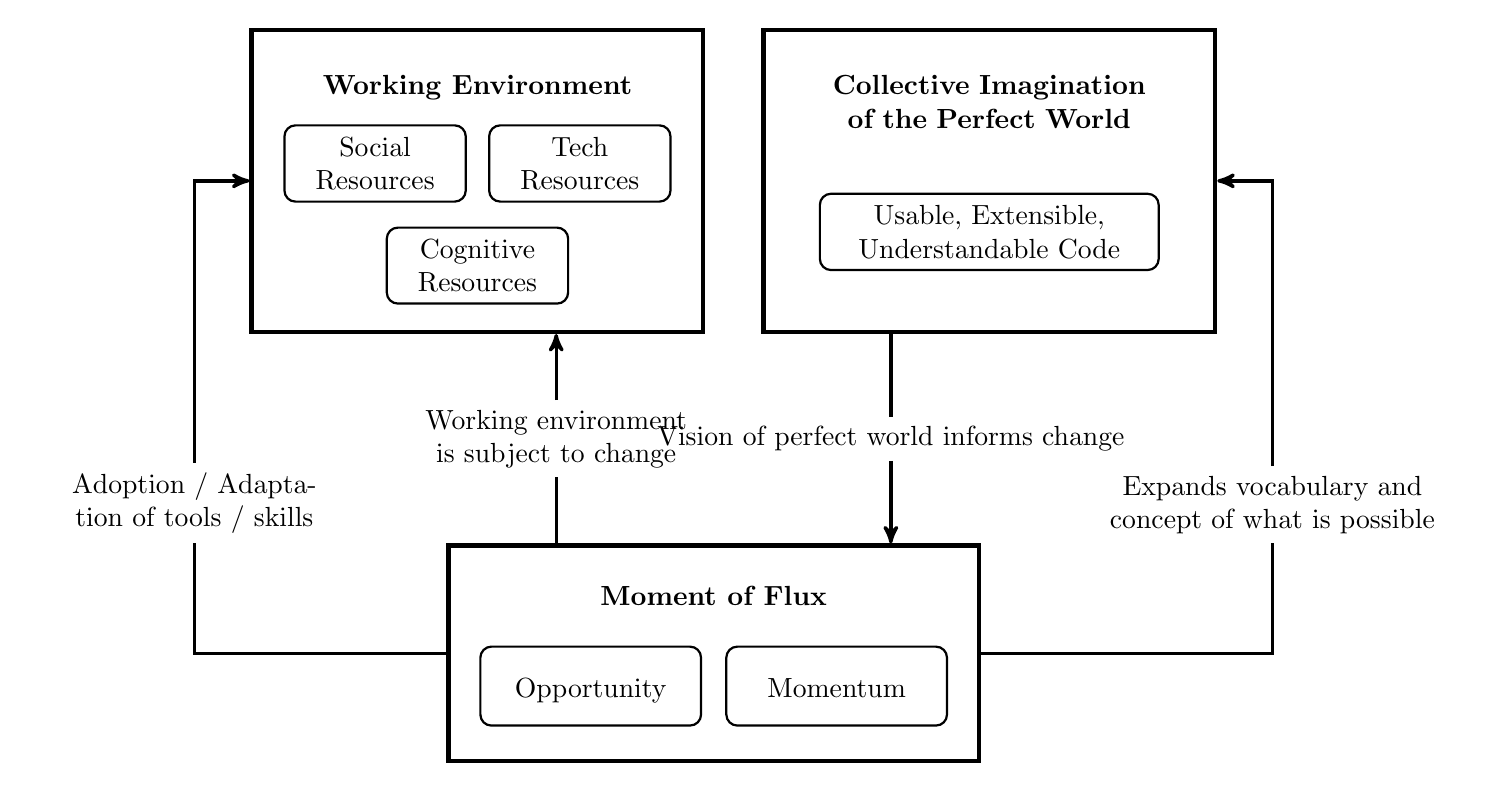
\begin{tikzpicture}[>=latex]
\usetikzlibrary{shapes,backgrounds,calc,arrows,positioning,arrows.meta}
\tikzset{>=stealth'}

\tikzstyle{bubble}=[draw, text centered, rounded corners, inner sep=1ex, thick]
\tikzstyle{cr}=[very thick]

% top left
\node(T1)[draw, text centered, ultra thick, text width=5.5cm, text height=3.6cm] at (0.5,0.5) {};
\node(T1t)[text centered, anchor=north] at ($(T1.north)!{(1/8)}!(T1.south)$) {\textbf{Working Environment}};

\node(T13)[style = bubble, text width=2cm] at ($(T1.north)!{(0.96-1.1/6)}!(T1.south)$) {Cognitive Resources};
\node(T11)[style = bubble, text width=2cm] at ($(T1.north)!{(0.96-3.1/6)}!(T1.south) - (1.3,0)$) {Social Resources};
\node(T12)[style = bubble, text width=2cm] at ($(T1.north)!{(0.96-3.1/6)}!(T1.south) + (1.3,0)$) {Tech Resources};


% top right
\node(S1)[draw, text centered, ultra thick, text width=5.5cm, text height=3.6cm] at (7,0.5) {};
\node(S1t)[text centered, anchor=north, text width = 5.5cm] at ($(S1.north)!{(1/8)}!(S1.south)$) {\textbf{Collective Imagination of the Perfect World}};

\node(S13)[style = bubble, text width=4cm] at ($(S1.north)!{(1-1/3)}!(S1.south)$) {Usable, Extensible, Understandable Code};


% low
\node(B1)[draw, text centered, ultra thick, text width=6.5cm, text height=2.5cm] at (3.5,-5.5) {};
\node(B1t)[text centered, anchor=north] at ($(B1.north)-(0, {(2.5*1/6)})$) {\textbf{Moment of Flux}};

\node(B11)[style = bubble, text width=2.5cm, text height=0.5cm, text depth=.2cm] at ($(B1.west)!0.27!(B1.east) + (0,-{(2.5*1/6)})$) {Opportunity};
\node(B12)[style = bubble, text width=2.5cm, text height=0.5cm, text depth=.2cm] at ($(B1.east)!0.27!(B1.west) + (0,-{(2.5*1/6)})$) {Momentum};


% text nodes
\node(R1)[text centered, text width = 4cm, anchor = south] at ($(B1.north -| T1.west) - (0.7,0)$) {Adoption / Adaptation of tools / skills};
\node(R2)[text centered, text width = 5cm, anchor = south] at ($(B1.north -| S1.east) + (0.7,0)$) {Expands vocabulary and concept of what is possible};

\node(R3)[text centered, text width = 6cm] at ($(B1.north)!0.5!(T1.south)-(0.5,0)$) {Working environment is subject to change};
\node(R4)[text centered, text width = 6cm] at ($(B1.north)!0.5!(S1.south)+(0.5,0)$) {Vision of perfect world informs change};

% arrows

\draw[->, style = cr] (B1) -| (R2) |- (S1);
\draw[->, style = cr] (B1) -| (R1) |- (T1);

\draw[->, style = cr] (B1.north -| R3) -- (R3) -- (T1.south -| R3);
\draw[->, style = cr] (S1.south -| R4) -- (R4) -- (B1.north -| R4);

\end{tikzpicture}